% =========================================================================
% WEEK 8: MAGNETOSTATICS I & II
% Master Lecture Transcript & Companion Guide
% =========================================================================

\section{Week 8: Magnetostatics (Lectures 13 \& 14)}
\label{sec:week8_master}

\subsection{Historical Foundations and Empirical Evidence}
\label{sec:intro_history}

For centuries, electrostatics and magnetism were viewed as entirely distinct natural phenomena. Electrostatics addressed stationary charges, mutual attraction or repulsion governed by Coulomb's law, and conservative electrostatic fields $\vb{E} = -\grad V$. Magnetism, by contrast, was historically observed in permanent natural magnets (lodestone, magnetite $\mathrm{Fe}_3\mathrm{O}_4$):
\begin{itemize}
    \item \textbf{Ancient Greece \& China:} Natural lodestones attract metallic iron but exert no net electrostatic force on noble metals such as gold or silver.
    \item \textbf{$12^{\mathrm{th}}$ Century Compass:} A suspended magnetic needle naturally aligns along the Earth's geomagnetic meridians, defining localized ``North'' and ``South'' poles. The fundamental empirical rule emerged: \emph{like poles repel, unlike poles attract}.
    \item \textbf{Absence of Isolated Magnetic Monopoles:} Cutting a magnetic diprotic bar in two does not isolate an independent North or South pole; rather, it produces two smaller dipoles.
\end{itemize}

\subsection{Oersted's Discovery and Ampère's Experiments}

In 1820, Hans Christian {\O}rsted discovered that an electric current flowing through a conductive wire deflected a nearby magnetic compass needle. This was the first empirical evidence coupling electricity and magnetism: \textbf{moving electric charges generate magnetic fields}.

Shortly thereafter, Andr\'e-Marie Amp\`ere systematically quantified the interaction forces between current-carrying conductors, demonstrating that:
\begin{enumerate}
    \item Two parallel wires carrying steady currents in the \textbf{same direction attract} one another.
    \item Two parallel wires carrying steady currents in \textbf{opposite directions repel} one another.
    \item A stationary electrostatic test charge placed adjacent to a current-carrying wire feels \textbf{no net force}, proving that the current-carrying conductor remains globally charge-neutral ($\rho = 0$).
\end{enumerate}

\begin{figure}[htbp]
    \centering
    \begin{tikzpicture}[scale=1.1, >=Stealth]
        % Left: Parallel (Attraction)
        \begin{scope}[shift={(0,0)}]
            \draw[very thick, ->] (0,-1.8) -- (0,1.8) node[below left=2pt] {$I_1$};
            \draw[very thick, ->] (2,-1.8) -- (2,1.8) node[below right=2pt] {$I_2$};
            
            % Attractive forces
            \draw[thick, ->, red!80!black] (0,0.6) -- (0.8,0.6) node[above, font=\footnotesize] {$\vb{F}$};
            \draw[thick, ->, red!80!black] (2,0.6) -- (1.2,0.6) node[above, font=\footnotesize] {$\vb{F}$};
            
            \draw[thick, ->, red!80!black] (0,-0.6) -- (0.8,-0.6);
            \draw[thick, ->, red!80!black] (2,-0.6) -- (1.2,-0.6);
            
            \node at (1,-2.3) {\small\textbf{Parallel: Attract}};
        \end{scope}

        % Right: Anti-parallel (Repulsion)
        \begin{scope}[shift={(5.5,0)}]
            \draw[very thick, ->] (0,-1.8) -- (0,1.8) node[below left=2pt] {$I_1$};
            \draw[very thick, <-] (2,-1.8) -- (2,1.8) node[above right=2pt] {$I_2$};
            
            % Repulsive forces
            \draw[thick, ->, red!80!black] (0,0.6) -- (-0.8,0.6) node[above, font=\footnotesize] {$\vb{F}$};
            \draw[thick, ->, red!80!black] (2,0.6) -- (2.8,0.6) node[above, font=\footnotesize] {$\vb{F}$};
            
            \draw[thick, ->, red!80!black] (0,-0.6) -- (-0.8,-0.6);
            \draw[thick, ->, red!80!black] (2,-0.6) -- (2.8,-0.6);
            
            \node at (1,-2.3) {\small\textbf{Anti-parallel: Repel}};
        \end{scope}
    \end{tikzpicture}
    \caption{Amp\`ere's experiment demonstrating the magnetic forces between parallel current filaments.}
    \label{fig:ampere_experiment}
\end{figure}

The physical cause of this magnetic interaction is mediated by the magnetic field $\vb{B}$: current $I_1$ establishes a circulating magnetic field $\vb{B}_1$, and the moving charges in wire 2 experience a magnetic force as they drift through $\vb{B}_1$.

\begin{figure}[htbp]
    \centering
    \begin{tikzpicture}[scale=1.1, >=Stealth]
        % Central wire carrying current
        \draw[very thick, ->] (0,-2.2) -- (0,2.2) node[above] {$I$};
        
        % Three concentric circulating loops
        \foreach \y in {-1.2, 0.0, 1.2} {
            \begin{scope}[shift={(0,\y)}]
                \draw[thick, color=Purple!70!black] (0,0) ellipse (1.6cm and 0.45cm);
                % Direction arrows along the ellipse
                \draw[thick, ->, color=Purple!70!black] (1.6,0) -- (1.6,0.05);
                \draw[thick, ->, color=Purple!70!black] (-1.6,0) -- (-1.6,-0.05);
                \draw[thick, ->, color=Purple!70!black] (0,-0.45) -- (0.1,-0.45);
            \end{scope}
        }
        \node[right, color=Purple!70!black] at (1.8,0) {$\vb{B}$ (circulating field)};
    \end{tikzpicture}
    \caption{The magnetic field $\vb{B}$ forms closed circulating loops around a current filament following the right-hand rule.}
    \label{fig:curling_b_field}
\end{figure}

---

\subsection{The Lorentz Force Law}
\label{sec:lorentz_force}

The fundamental empirical law defining both electric and magnetic fields acting on an arbitrary test particle of charge $Q$ moving with velocity $\vb{v}$ is the \textbf{Lorentz Force Law}.

\begin{definition}{Lorentz Force}{lorentz_force}
A point particle with electric charge $Q$ moving with instantaneous velocity $\vb{v}$ in an electromagnetic field $(\vb{E}, \vb{B})$ experiences the total vector force:
\begin{equation}
    \vb{F} = Q\qty(\vb{E} + \vb{v} \times \vb{B})
    \label{eq:lorentz_law}
\end{equation}
The purely magnetic contribution is:
\begin{equation}
    \vb{F}_{\mathrm{mag}} = Q\qty(\vb{v} \times \vb{B})
    \label{eq:magnetic_force}
\end{equation}
\end{definition}

\begin{figure}[htbp]
    \centering
    \begin{tikzpicture}[scale=1.1, >=Stealth]
        % Shaded plane
        \fill[SeaGreen!10] (-2.2,-0.5) -- (1.5,-0.5) -- (3.2,1.2) -- (-0.5,1.2) -- cycle;
        \draw[thin, SeaGreen!60!black] (-2.2,-0.5) -- (1.5,-0.5) -- (3.2,1.2) -- (-0.5,1.2) -- cycle;
        
        % Vectors at the origin in the plane
        \coordinate (O) at (0.4,0.2);
        \draw[fill=black] (O) circle (1.8pt) node[below right] {$q > 0$};
        
        \draw[very thick, ->, red!80!black] (O) -- ++(-1.6,-0.3) node[below left] {$\vb{v}$};
        \draw[very thick, ->, Cyan!80!black] (O) -- ++(-1.2,0.4) node[above left] {$\vb{B}$};
        
        % Angle arc
        \draw[thin] (O) ++(-0.6,-0.11) arc (-170:-145:0.7);
        \node at ($(O)+(-0.8,0.05)$) {\footnotesize $\theta$};
        
        % Force vector perpendicular to the plane
        \draw[ultra thick, ->, Blue!80!black] (O) -- ++(0,2.0) node[above] {$\vb{F}_{\mathrm{mag}} = q(\vb{v}\times\vb{B})$};
    \end{tikzpicture}
    \caption{The magnetic force vector $\vb{F}_{\mathrm{mag}}$ is strictly perpendicular to the plane spanned by $\vb{v}$ and $\vb{B}$.}
    \label{fig:f_v_b_geometry}
\end{figure}

\subsection{Key Physical Consequences of the Magnetic Force}
\begin{enumerate}
    \item \textbf{Directional Geometry:} Since $\vb{F}_{\mathrm{mag}} = Q(\vb{v} \times \vb{B})$, the force is normal to both the instantaneous velocity $\vb{v}$ and the field $\vb{B}$. If $\vb{v} \parallel \vb{B}$, the magnetic force identically vanishes ($\abs{\vb{F}} \propto \sin\theta = 0$).
    \item \textbf{SI Dimensional Analysis \& Units:}
    \begin{equation}
        [B] = \frac{[F]}{[Q][v]} = \frac{\mathrm{N}}{\mathrm{C} \cdot \mathrm{m}/\mathrm{s}} = \frac{\mathrm{N}}{\mathrm{A} \cdot \mathrm{m}} \equiv \mathrm{Tesla}\ (\mathrm{T})
    \end{equation}
    In cgs-Gaussian units, the unit of magnetic flux density is the \textbf{Gauss} ($\mathrm{G}$):
    \begin{equation}
        1\ \mathrm{T} = 10^4\ \mathrm{Gauss}
    \end{equation}
    Typical values: Earth's magnetic surface field $\sim 0.5\ \mathrm{G} = 5 \times 10^{-5}\ \mathrm{T}$; strong laboratory superconducting electromagnets $\sim 1\text{--}15\ \mathrm{T}$.
\end{enumerate}

\begin{theorem}{Work Done by Magnetic Forces}{magnetic_work}
The magnetic force does \textbf{zero mechanical work} on any moving charged particle:
\begin{equation}
    W_{\mathrm{mag}} = \int \vb{F}_{\mathrm{mag}} \cdot d\vb{\ell} = 0
\end{equation}
\end{theorem}

\begin{proofbox}
Consider the differential mechanical work done by $\vb{F}_{\mathrm{mag}}$ in time interval $dt$:
\begin{equation}
    dW_{\mathrm{mag}} = \vb{F}_{\mathrm{mag}} \cdot d\vb{\ell} = \vb{F}_{\mathrm{mag}} \cdot (\vb{v}\,dt) = Q\qty(\vb{v} \times \vb{B}) \cdot \vb{v}\,dt
\end{equation}
By the algebraic properties of the scalar triple product, the vector $(\vb{v} \times \vb{B})$ is orthogonal to $\vb{v}$. Consequently, the inner product identically evaluates to zero:
\begin{equation}
    (\vb{v} \times \vb{B}) \cdot \vb{v} = 0 \implies dW_{\mathrm{mag}} = 0 \implies \dv{K}{t} = \vb{F} \cdot \vb{v} = 0
\end{equation}
where $K = \frac{1}{2}m v^2$ is the kinetic energy of the charge carrier.
\end{proofbox}

\begin{remark}
A static magnetic field can alter the \textbf{direction} of a particle's linear momentum, but it cannot change its kinetic energy or scalar speed $v = \abs{\vb{v}}$.
\end{remark}

---

\subsection{Charged Particle Trajectories in Static Magnetic Fields}
\label{sec:particle_trajectories}

\subsubsection{Uniform Magnetic Field: Pure Cyclotron Motion}

Let a non-relativistic particle of mass $m$ and positive charge $q > 0$ enter a region of uniform magnetic field oriented perpendicular to its initial velocity vector:
\begin{equation}
    \vb{B} = -B\,\vu{z} \quad (\text{pointing into the page}), \qquad \vb{v}_0 = v\,\vu{x}
\end{equation}

\begin{figure}[htbp]
    \centering
    \begin{tikzpicture}[scale=1.1, >=Stealth]
        % Axes
        \draw[thin, ->] (-2.6,0) -- (2.8,0) node[right] {$x$};
        \draw[thin, ->] (0,-2.6) -- (0,2.8) node[above] {$y$};
        \draw[thin, ->] (0,0) -- (-1.5,-1.5) node[below left] {$z$};

        % Circular orbit
        \draw[thick, Purple] (0,0) circle (1.8cm);

        % Positions and vectors
        % At (1.8, 0)
        \draw[fill=blue] (1.8,0) circle (2pt);
        \draw[thick, ->, OliveGreen] (1.8,0) -- (1.8,0.9) node[above right] {$\vb{v}$};
        \draw[thick, ->, Blue] (1.8,0) -- (0.9,0) node[above] {$\vb{F}_{\mathrm{mag}}$};

        % At (0, 1.8)
        \draw[fill=blue] (0,1.8) circle (2pt);
        \draw[thick, ->, OliveGreen] (0,1.8) -- (-0.9,1.8) node[above left] {$\vb{v}$};
        \draw[thick, ->, Blue] (0,1.8) -- (0,0.9) node[left] {$\vb{F}_{\mathrm{mag}}$};

        % At (-1.8, 0)
        \draw[fill=blue] (-1.8,0) circle (2pt);
        \draw[thick, ->, OliveGreen] (-1.8,0) -- (-1.8,-0.9) node[below left] {$\vb{v}$};
        \draw[thick, ->, Blue] (-1.8,0) -- (-0.9,0) node[below] {$\vb{F}_{\mathrm{mag}}$};

        % At (0, -1.8)
        \draw[fill=blue] (0,-1.8) circle (2pt);
        \draw[thick, ->, OliveGreen] (0,-1.8) -- (0.9,-1.8) node[below right] {$\vb{v}$};
        \draw[thick, ->, Blue] (0,-1.8) -- (0,-0.9) node[right] {$\vb{F}_{\mathrm{mag}}$};

        \node[font=\footnotesize, Blue] at (0.4,0.4) {$\vb{F}_{\mathrm{centripetal}}$};
    \end{tikzpicture}
    \caption{Uniform circular motion of a positive charge $q>0$ subjected to a perpendicular uniform field $\vb{B} = -B\,\vu{z}$.}
    \label{fig:cyclotron_orbit}
\end{figure}

The instantaneous magnetic force provides the required centripetal acceleration:
\begin{equation}
    F_{\mathrm{mag}} = q v B = \frac{m v^2}{R}
\end{equation}
Solving for the \textbf{cyclotron radius} (gyroradius) $R$:
\begin{equation}
    R = \frac{m v}{\abs{q} B}
    \label{eq:cyclotron_radius}
\end{equation}
The period $T$ of one complete orbit and the fundamental \textbf{cyclotron frequency} $\omega_c$ are:
\begin{equation}
    T = \frac{2\pi R}{v} = \frac{2\pi m}{\abs{q} B}, \qquad \omega_c = \frac{2\pi}{T} = \frac{\abs{q} B}{m}
    \label{eq:cyclotron_freq}
\end{equation}

\begin{remark}
Crucially, the orbital period $T$ and angular frequency $\omega_c$ are \textbf{independent of velocity} $v$. Faster particles trace wider geometric circles, but traverse them in the exact same elapsed duration. This is the operational foundation of Ernest Lawrence's particle \textbf{cyclotron}.
\end{remark}

\subsubsection{General Helical Trajectory}

If the particle's initial velocity has a component parallel to the uniform magnetic field $\vb{B} = B\,\vu{z}$, we decompose $\vb{v} = \vb{v}_{\parallel} + \vb{v}_{\perp}$:
\begin{itemize}
    \item Along $\vu{z}$: $\vb{F}_{\parallel} = q(\vb{v}_{\parallel} \times \vb{B}) = 0 \implies v_z(t) = \text{const}$.
    \item Transverse plane $(x,y)$: $\vb{F}_{\perp} = q(\vb{v}_{\perp} \times \vb{B})$ executes uniform circular motion with gyroradius $R = \frac{m v_{\perp}}{\abs{q} B}$.
\end{itemize}

Superposing uniform linear translation with perpendicular circular motion yields a continuous \textbf{helix} along the magnetic field line.

\begin{figure}[htbp]
    \centering
    \begin{tikzpicture}[scale=1.1, >=Stealth]
        % Axes
        \draw[thin, ->] (0,0,0) -- (3.2,0,0) node[below] {$y$};
        \draw[thin, ->] (0,0,0) -- (0,3.6,0) node[left] {$z$};
        \draw[thin, ->] (0,0,0) -- (0,0,3.0) node[below left] {$x$};
        
        % Uniform B field vectors
        \foreach \x in {1.2, 1.5, 1.8} {
            \draw[thick, ->, PineGreen] (\x,0.4) -- (\x,3.2);
        }
        \node[PineGreen, right] at (1.8,3.0) {$\vb{B}$};
        
        % Helix parametrization
        \draw[very thick, Purple, domain=0:5.2*pi, samples=200, variable=\t]
            plot ({1.5 + 0.5*cos(\t r)}, {0.5 + 0.16*\t}, {0.5*sin(\t r)});
            
        \node[Purple, right] at (2.1,2.0) {Helical path};
        \fill[Purple] ({1.5 + 0.5*cos(0)}, 0.5, 0) circle (2.2pt) node[right, font=\footnotesize] {$q^+$};
    \end{tikzpicture}
    \caption{Helical trajectory produced when the initial particle velocity possesses a non-zero component $v_{\parallel}$ along the ambient magnetic field $\vb{B}$.}
    \label{fig:helical_motion}
\end{figure}

The spatial distance between adjacent turns is the \textbf{pitch} $p$ of the helix:
\begin{equation}
    p = v_{\parallel} T = v_{\parallel} \frac{2\pi m}{\abs{q} B}
\end{equation}

---

\subsection{Velocity Selectors and the Thomson $e/m$ Experiment}
\label{sec:thomson_experiment}

In 1897, J.~J.~Thomson evaluated the charge-to-mass ratio of the electron using crossed electric and magnetic fields, conclusively discovering subatomic charged constituents.

\begin{example}[Crossed Field Velocity Filter]
Consider mutually perpendicular uniform fields $\vb{E} = -E\,\vu{y}$ and $\vb{B} = -B\,\vu{z}$ (pointing into the page). An electron beam ($q = -e$) is accelerated from rest across an electrostatic potential difference $\Delta V = V_A - V_C$:
\begin{equation}
    \Delta K = \frac{1}{2}m v^2 = e \Delta V \implies v = \sqrt{\frac{2e\Delta V}{m}}
\end{equation}
Upon entering the crossed field region, the total transverse Lorentz force is:
\begin{equation}
    \vb{F} = q\qty(\vb{E} + \vb{v}\times \vb{B}) = -e\qty(-E\,\vu{y} + (v\,\vu{x})\times(-B\,\vu{z})) = e\qty(E - v B)\vu{y}
\end{equation}
To achieve undeflected, rectilinear transmission through the aperture:
\begin{equation}
    \vb{F} = \vb{0} \iff E = v B \implies v = \frac{E}{B}
\end{equation}
Only particles with this precise velocity pass through without deflection. Equating the two velocity expressions:
\begin{equation}
    \frac{E}{B} = \sqrt{\frac{2e\Delta V}{m}} \implies \frac{e}{m} = \frac{E^2}{2 \Delta V B^2} \approx 1.7588 \times 10^{11}\ \mathrm{C/kg}
\end{equation}
\end{example}

---

\subsection{Magnetic Forces on Current-Carrying Conductors}
\label{sec:forces_on_wires}

Consider a macroscopic conductor carrying electric current $I$. The total current is given by $I = n q v_d A$, where $n$ is charge carrier number density, $q$ is charge per carrier, $v_d$ is the drift velocity, and $A$ is the cross-sectional area.

\begin{figure}[htbp]
    \centering
    \begin{tikzpicture}[scale=1.1, >=Stealth]
        % B field background crosses
        \foreach \x in {-1.8, -1.0, -0.2, 0.6, 1.4, 2.2} {
            \foreach \y in {-1.2, -0.4, 0.4, 1.2} {
                \node[gray!60] at (\x,\y) {$\times$};
            }
        }
        \node[font=\bfseries, right] at (2.3,0.5) {$\vb{B}$ (into page)};

        % Wire segment
        \draw[thick, fill=Emerald!15] (-0.3,-1.4) rectangle (0.3,1.4);
        \node[above] at (0,1.4) {$A$};
        
        % Drift velocity and Force
        \draw[very thick, ->, Purple] (0,-0.8) -- (0,0.8) node[midway, right] {$\vb{v}_d,\ I$};
        \draw[ultra thick, ->, red!85!black] (0,0.2) -- (-1.2,0.2) node[above] {$\vb{F}$};
        
        % Dimension bracket
        \draw[<->] (0.5,-1.4) -- (0.5,1.4) node[midway, right] {$\ell$};
    \end{tikzpicture}
    \caption{A conducting segment of length $\ell$ carrying current $I$ in a transverse field $\vb{B}$.}
    \label{fig:wire_segment_force}
\end{figure}

The net force on a wire segment of length $\vb{L} = \ell\,\vu{t}$ is:
\begin{equation}
    \vb{F}_{\mathrm{mag}} = \sum Q_i (\vb{v}_d \times \vb{B}) = (n A \ell q) (\vb{v}_d \times \vb{B}) = I(\vb{L} \times \vb{B})
\end{equation}
For an arbitrary, curved wire spanning from anchor point $a$ to $b$, the total force is the line integral over differential elements $d\vb{s}$:
\begin{equation}
    \vb{F}_{\mathrm{mag}} = I \int_{a}^{b} d\vb{s} \times \vb{B}
    \label{eq:force_wire_integral}
\end{equation}

\begin{proposition}{Uniform Field Properties}{uniform_b_force}
If the ambient magnetic field $\vb{B}$ is spatially uniform:
\begin{enumerate}
    \item For any open wire between endpoints $a$ and $b$, the force depends exclusively on the end-to-end vector $\vb{L} = \int_{a}^{b} d\vb{s}$:
    \begin{equation}
        \vb{F}_{\mathrm{mag}} = I \qty(\int_{a}^{b} d\vb{s}) \times \vb{B} = I (\vb{L} \times \vb{B})
    \end{equation}
    \item For \textbf{any closed current loop} $\mathcal{C}$ in a uniform magnetic field $\vb{B}$, the net magnetic force is identically zero:
    \begin{equation}
        \vb{F}_{\mathrm{net}} = I \qty(\oint_{\mathcal{C}} d\vb{s}) \times \vb{B} = \vb{0}
    \end{equation}
    since the contour integral of displacement around a closed loop vanishes: $\oint_{\mathcal{C}} d\vb{s} = \vb{0}$.
\end{enumerate}
\end{proposition}

\begin{example}[Semi-Circular Loop in a Transverse Field]
Consider a closed planar circuit in the $xy$-plane consisting of a straight segment along the $x$-axis from $x = -R$ to $x = +R$ and a semi-circular arc of radius $R$ in the upper half-plane, carrying current $I$ counter-clockwise in a uniform field $\vb{B} = B\,\vu{y}$.

\begin{center}
\begin{tikzpicture}[scale=1.1, >=Stealth]
    \draw[thin, ->] (-2.5,0) -- (2.8,0) node[right] {$x$};
    \draw[thin, ->] (0,-0.5) -- (0,2.6) node[above] {$y$};
    
    % Field vector
    \draw[thick, ->, Blue] (-2.2,0.8) -- (-2.2,2.0) node[above] {$\vb{B} = B\,\vu{y}$};
    
    % Semicircle
    \draw[very thick, ForestGreen, domain=0:180, samples=100] plot ({1.8*cos(\x)}, {1.8*sin(\x)});
    \draw[very thick, ForestGreen, ->] (-1.8,0) -- (0.2,0);
    \draw[very thick, ForestGreen] (0,0) -- (1.8,0);
    
    % Arrows along arc
    \draw[very thick, ->, ForestGreen] ({1.8*cos(45)}, {1.8*sin(45)}) -- ++({-0.1*sin(45)}, {0.1*cos(45)});
    \draw[very thick, ->, ForestGreen] ({1.8*cos(135)}, {1.8*sin(135)}) -- ++({-0.1*sin(135)}, {0.1*cos(135)});
    
    % Polar elements
    \draw[dashed] (0,0) -- ({1.8*cos(35)}, {1.8*sin(35)});
    \draw[dashed] (0,0) -- ({1.8*cos(55)}, {1.8*sin(55)});
    \draw[thin] (0.5,0) arc (0:35:0.5) node[midway, right=1pt] {\footnotesize $\theta$};
    \draw[thin] (0.9,0.5) arc (35:55:0.9) node[midway, above right] {\footnotesize $d\theta$};
    \node at (1.0,1.0) {$R$};
\end{tikzpicture}
\end{center}

\textbf{1. Straight segment ($a = -R$ to $b = +R$):}
\begin{equation}
    \vb{F}_1 = I \vb{L} \times \vb{B} = I (2R\,\vu{x}) \times (B\,\vu{y}) = 2IRB\,\vu{z}
\end{equation}
\textbf{2. Semi-circular arc:} The element $d\vb{s} = R\,d\theta(-\sin\theta\,\vu{x} + \cos\theta\,\vu{y})$.
\begin{equation}
    d\vb{F}_2 = I d\vb{s} \times \vb{B} = I R\,d\theta\qty(-\sin\theta\,\vu{x} + \cos\theta\,\vu{y}) \times (B\,\vu{y}) = -IRB\sin\theta\,d\theta\,\vu{z}
\end{equation}
Integrating from $\theta = 0$ to $\pi$:
\begin{equation}
    \vb{F}_2 = -IRB\,\vu{z} \int_{0}^{\pi} \sin\theta\,d\theta = -IRB\,\vu{z} \qty[-\cos\theta]_0^\pi = -2IRB\,\vu{z}
\end{equation}
Summing the components confirms that the net force vanishes:
\begin{equation}
    \vb{F}_{\mathrm{net}} = \vb{F}_1 + \vb{F}_2 = 2IRB\,\vu{z} - 2IRB\,\vu{z} = \vb{0}
\end{equation}
\end{example}

---

\subsection{Magnetic Torques and Magnetic Dipole Moments}
\label{sec:magnetic_torques}

Although the net translational force on a closed planar current loop in a uniform field is zero, the forces acting on opposite sides produce a net \textbf{mechanical torque}.

\subsubsection{Derivation for a Rectangular Loop}

Consider a planar rectangular loop of dimensions $a \times b$ in the $xy$-plane carrying current $I$ in a uniform magnetic field $\vb{B} = B\,\vu{x}$.

\begin{figure}[htbp]
    \centering
    \begin{tikzpicture}[scale=1.1, >=Stealth]
        % Perspective coordinates
        \draw[thin, ->] (-0.5,0) -- (4.2,0) node[right] {$x$};
        \draw[thin, ->] (0,-0.5) -- (0,2.2) node[above] {$z$};
        \draw[thin, ->] (0,0) -- (-1.2,-1.2) node[below left] {$y$};
        
        % Rectangular loop
        \coordinate (P1) at (0.4,0.3);
        \coordinate (P2) at (3.2,0.3);
        \coordinate (P3) at (2.4,-0.8);
        \coordinate (P4) at (-0.4,-0.8);
        
        \draw[very thick, ForestGreen] (P1) -- (P2) node[midway, above] {$b$, (1)}
                                    -- (P3) node[midway, right] {$a$, (4)}
                                    -- (P4) node[midway, below] {$b$, (3)}
                                    -- (P1) node[midway, left] {$a$, (2)};
                                    
        % Currents
        \draw[thick, ->, ForestGreen] (P2) -- ($(P1)!0.5!(P2)$);
        \draw[thick, ->, ForestGreen] (P3) -- ($(P2)!0.5!(P3)$);
        \draw[thick, ->, ForestGreen] (P4) -- ($(P3)!0.5!(P4)$);
        \draw[thick, ->, ForestGreen] (P1) -- ($(P4)!0.5!(P1)$);

        % Magnetic Field
        \draw[ultra thick, ->, Blue] (1.0,-1.6) -- (2.8,-1.6) node[midway, below] {$\vb{B} = B\,\vu{x}$};

        % Forces on sides (2) and (4)
        \draw[ultra thick, ->, red!85!black] (P1) -- ++(0,1.2) node[above] {$\vb{F}_2$};
        \draw[ultra thick, ->, red!85!black] (P3) -- ++(0,-1.2) node[below] {$\vb{F}_4$};
    \end{tikzpicture}
    \caption{Rectangular current loop subjected to a uniform field $\vb{B}$, illustrating the couple $\vb{F}_2, \vb{F}_4$.}
    \label{fig:torque_loop}
\end{figure}

Evaluating the force on each segment:
\begin{align}
    \vb{F}_1 &= I(-b\,\vu{x}) \times (B\,\vu{x}) = \vb{0} \\
    \vb{F}_3 &= I(b\,\vu{x}) \times (B\,\vu{x}) = \vb{0} \\
    \vb{F}_2 &= I(-a\,\vu{y}) \times (B\,\vu{x}) = +IaB\,\vu{z} \\
    \vb{F}_4 &= I(a\,\vu{y}) \times (B\,\vu{x}) = -IaB\,\vu{z}
\end{align}
Taking the origin at the center of the loop, the lever-arm vectors to sides 2 and 4 are $\vb{r}_2 = -\frac{b}{2}\,\vu{x}$ and $\vb{r}_4 = +\frac{b}{2}\,\vu{x}$. The torque is:
\begin{equation}
    \bm{\tau} = \vb{r}_2 \times \vb{F}_2 + \vb{r}_4 \times \vb{F}_4 = \qty(-\frac{b}{2}\,\vu{x}) \times (IaB\,\vu{z}) + \qty(\frac{b}{2}\,\vu{x}) \times (-IaB\,\vu{z}) = I a b B\,\vu{y} = I A B\,\vu{y}
\end{equation}
where $A = ab$ is the area enclosed by the loop.

\begin{figure}[htbp]
    \centering
    \begin{tikzpicture}[scale=1.1, >=Stealth]
        % Edge on view: loop rotated by angle theta
        \coordinate (O) at (0,0);
        \draw[fill=black] (O) circle (1.8pt);
        
        % Axes
        \draw[thin, ->] (O) -- (3.0,0) node[right] {$\vb{B}$ (along $x$)};
        \draw[thin, ->] (O) -- (0,2.5) node[above] {$z$};
        \draw[thin] (O) circle (4pt);
        \draw[fill=black] (O) circle (1pt);
        \node[below left] at (O) {$y$ (out of page)};
        
        % Rotated loop line
        \coordinate (A2) at (-1.2,1.6);
        \coordinate (A4) at (1.2,-1.6);
        \draw[very thick] (A2) -- (A4);
        
        % Force vectors
        \draw[ultra thick, ->, Blue] (A2) -- ++(0,1.4) node[above] {$\vb{F}_2$};
        \draw[ultra thick, ->, Blue] (A4) -- ++(0,-1.4) node[below] {$\vb{F}_4$};
        
        % Current markers
        \draw (A2) circle (3.5pt); \fill (A2) circle (1.5pt); % current out
        \draw (A4) circle (3.5pt); \draw (A4) ++(-2.5pt,-2.5pt) -- ++(5pt,5pt); \draw (A4) ++(-2.5pt,2.5pt) -- ++(5pt,-5pt); % current in
        
        % Lever arm labels
        \draw[dashed, ->] (O) -- (A2) node[midway, left] {$\vb{r}_2$};
        \draw[dashed, ->] (O) -- (A4) node[midway, right] {$\vb{r}_4$};
        
        % Area normal vector and angle
        \draw[very thick, ->, ForestGreen] (O) -- (1.5,1.125) node[above right] {$\bm{\mu} = I\vb{A}$};
        \draw[thin] (0.8,0) arc (0:37:0.8) node[midway, right] {\footnotesize $\theta$};
    \end{tikzpicture}
    \caption{Edge-on view: the area normal vector $\vb{A}$ forms an angle $\theta$ with the ambient field $\vb{B}$.}
    \label{fig:edge_on_torque}
\end{figure}

\begin{definition}{Magnetic Dipole Moment and General Torque}{magnetic_dipole}
For a planar loop of area $A$ carrying current $I$ with $N$ turns, the \textbf{magnetic dipole moment} is:
\begin{equation}
    \bm{\mu} \equiv N I \vb{A} = N I A\,\vu{n}
    \label{eq:magnetic_dipole_def}
\end{equation}
where $\vu{n}$ is the unit normal vector given by the right-hand rule curled along $I$. The torque on the loop is:
\begin{equation}
    \bm{\tau} = \bm{\mu} \times \vb{B}
    \label{eq:torque_mu_cross_b}
\end{equation}
The potential energy associated with orienting the dipole is:
\begin{equation}
    U = -\bm{\mu} \cdot \vb{B}
\end{equation}
\end{definition}

---

\subsection{Steady Currents and the Biot-Savart Law}
\label{sec:biot_savart_law}

\subsubsection{Physical Nature of Steady Currents}

In magnetostatics, the fundamental source is a \textbf{steady current}. By definition, steady currents exhibit time-invariant current density:
\begin{equation}
    \pdv{\vb{J}}{t} = \vb{0}
\end{equation}
From the continuity equation of electrodynamics:
\begin{equation}
    \div\vb{J} + \pdv{\rho}{t} = 0
\end{equation}
If charge does not accumulate anywhere in the steady state, $\pdv{\rho}{t} = 0$, leading to:
\begin{equation}
    \div\vb{J} = 0
    \label{eq:continuity_steady}
\end{equation}
Hence, steady current lines never start nor terminate; they form closed continuous paths.

\subsubsection{The Biot-Savart Law}

\begin{definition}{The Biot-Savart Law}{biot_savart}
An infinitesimal line element $d\vb{s}$ of a wire carrying a steady current $I$ produces a differential magnetic field $d\vb{B}$ at observation point $P$:
\begin{equation}
    d\vb{B}(P) = \frac{\mu_0}{4\pi} \frac{I\,d\vb{s} \times \vu{r}^*}{{r^*}^2} = \frac{\mu_0}{4\pi} \frac{I\,d\vb{s} \times \vb{r}^*}{{r^*}^3}
    \label{eq:biot_savart_line}
\end{equation}
where:
\begin{itemize}
    \item $\mu_0 \equiv 4\pi \times 10^{-7}\ \mathrm{T\cdot m / A}$ is the \textbf{permeability of free space}.
    \item $\vb{r}^* \equiv \vb{r}_P - \vb{r}'$ is the separation vector from source to field point, with $r^* = \abs{\vb{r}^*}$ and $\vu{r}^* = \vb{r}^*/r^*$.
\end{itemize}
The total field is obtained by integrating along the entire wire circuit:
\begin{equation}
    \vb{B}(\vb{r}_P) = \frac{\mu_0 I}{4\pi} \int_{\mathrm{wire}} \frac{d\vb{s} \times \vu{r}^*}{{r^*}^2}
\end{equation}
\end{definition}

\begin{figure}[htbp]
    \centering
    \begin{tikzpicture}[scale=1.1, >=Stealth]
        % Current wire curve
        \draw[very thick, ForestGreen] (-1.5,-0.5) to[out=20, in=200] (0,0) to[out=20, in=190] (3.0,0.4);
        \draw[thick, ->, ForestGreen] (2.0,0.3) -- (2.4,0.36) node[below right] {$I$};

        % Source segment ds
        \coordinate (S) at (0,0);
        \draw[fill=black] (S) circle (1.5pt);
        \draw[ultra thick, ->, black] (S) -- (0.8,0.2) node[below right] {$d\vb{s}$};

        % Field point P
        \coordinate (P) at (2.0,2.5);
        \draw[fill=black] (P) circle (1.8pt) node[above right] {$P$};

        % Separation vector r*
        \draw[thick, ->, Purple] (S) -- (P) node[midway, left] {$\vb{r}^* = \vb{r}_P - \vb{r}'$};
        \draw[very thick, ->, PineGreen] (S) -- ($(S)!0.38!(P)$) node[above left] {$\vu{r}^*$};
    \end{tikzpicture}
    \caption{Geometric configuration of the Biot-Savart law: source segment $d\vb{s}$ and separation vector $\vb{r}^*$.}
    \label{fig:biot_savart_geom}
\end{figure}

---

\subsection{Applications of the Biot-Savart Law}
\label{sec:biot_savart_applications}

\subsubsection{Magnetic Field on the Axis of a Circular Current Loop}

Consider a circular ring of radius $R$ positioned in the $xy$-plane centered at the origin, carrying a steady current $I$ counter-clockwise as viewed from $+z$. We compute the magnetic field at an axial point $P = (0, 0, z)$.

\begin{figure}[htbp]
    \centering
    \begin{tikzpicture}[scale=1.1, >=Stealth]
        % 3D Axes
        \draw[thin, ->] (0,0) -- (0,3.6) node[above] {$z$};
        \draw[thin, ->] (0,0) -- (3.2,0) node[right] {$y$};
        \draw[thin, ->] (0,0) -- (-1.8,-1.5) node[below left] {$x$};
        
        % Ring in xy plane
        \draw[thick, ForestGreen] (0,0) ellipse (2.2cm and 0.7cm);
        \draw[thick, ->, ForestGreen] (-2.2,0) arc (180:220:2.2cm and 0.7cm) node[below left] {$I$};

        % Source point on ring
        \coordinate (SP) at (1.4,-0.54);
        \draw[fill=Purple] (SP) circle (2pt) node[below right] {$I\,d\vb{s}$};
        \draw[thick, ->, Purple] (SP) -- ++(0.7,0.18) node[above right] {$d\vb{s}$};
        
        % Vector r'
        \draw[thick, ->, Purple!80!black] (0,0) -- (SP) node[midway, below] {$\vb{r}'$};

        % Observation Point P
        \coordinate (OP) at (0,2.6);
        \draw[fill=blue] (OP) circle (2pt) node[left] {$P(0,0,z)$};
        \draw[thick, ->, Blue] (0,0) -- (OP) node[midway, left] {$\vb{r}_P = z\vu{z}$};

        % Separation vector r*
        \draw[very thick, ->, Cyan!80!black] (SP) -- (OP) node[midway, right] {$\vb{r}^*$};
    \end{tikzpicture}
    \caption{Coordinate framework for integrating the magnetic field of a circular current loop on its symmetry axis.}
    \label{fig:loop_axis_cartesian}
\end{figure}

\paragraph{Method 1: Direct Cartesian Integration}
\begin{enumerate}
    \item \textbf{Source position:} Using azimuthal angle $\phi' \in [0, 2\pi]$:
    \begin{equation}
        \vb{r}' = R\cos\phi'\,\vu{x} + R\sin\phi'\,\vu{y} \implies d\vb{s} = R\,d\phi'\qty(-\sin\phi'\,\vu{x} + \cos\phi'\,\vu{y})
    \end{equation}
    \item \textbf{Field position:} $\vb{r}_P = z\,\vu{z}$.
    \item \textbf{Separation vector:}
    \begin{equation}
        \vb{r}^* = \vb{r}_P - \vb{r}' = -R\cos\phi'\,\vu{x} - R\sin\phi'\,\vu{y} + z\,\vu{z}, \qquad r^* = \sqrt{R^2 + z^2}
    \end{equation}
    \item \textbf{Vector cross product:}
    \begin{equation}
        d\vb{s} \times \vb{r}^* = R\,d\phi'\mqty| \vu{x} & \vu{y} & \vu{z} \\ -\sin\phi' & \cos\phi' & 0 \\ -R\cos\phi' & -R\sin\phi' & z | = R\,d\phi'\qty[z\cos\phi'\,\vu{x} + z\sin\phi'\,\vu{y} + R\,\vu{z}]
    \end{equation}
    \item \textbf{Integration:}
    \begin{align}
        B_x &= \frac{\mu_0 I R z}{4\pi (R^2+z^2)^{3/2}} \int_0^{2\pi} \cos\phi'\,d\phi' = 0 \\
        B_y &= \frac{\mu_0 I R z}{4\pi (R^2+z^2)^{3/2}} \int_0^{2\pi} \sin\phi'\,d\phi' = 0 \\
        B_z &= \frac{\mu_0 I R^2}{4\pi (R^2+z^2)^{3/2}} \int_0^{2\pi} d\phi' = \frac{\mu_0 I R^2}{2(R^2+z^2)^{3/2}}
    \end{align}
\end{enumerate}

\paragraph{Method 2: Symmetry and Geometric Cone Analysis}

\begin{figure}[htbp]
    \centering
    \begin{tikzpicture}[scale=1.1, >=Stealth]
        % Vertical z-axis
        \draw[thin, ->] (0,-0.8) -- (0,3.6) node[above] {$z$};
        
        % Ring
        \draw[thick, ForestGreen] (0,0) ellipse (1.6cm and 0.4cm);
        \draw[dashed] (-1.6,0) -- (0,0) node[midway, above] {$R$};
        
        % Point P
        \coordinate (P) at (0,2.0);
        \draw[fill=blue] (P) circle (1.8pt) node[left] {$P$};
        
        % Slanted lines to loop edge
        \draw[thick] (P) -- (1.6,0) node[midway, right] {$r^*$};
        \draw[thick] (P) -- (-1.6,0);
        
        % dB vectors forming a cone
        \draw[dashed] (0,2.6) ellipse (1.0cm and 0.25cm);
        \draw[very thick, ->, Blue] (P) -- (0.8,2.6) node[above right] {$d\vb{B}$};
        \draw[very thick, ->, Blue] (P) -- (-0.8,2.6);
        \draw[ultra thick, ->, Purple] (P) -- (0,3.2) node[right] {$\vb{B}_{\mathrm{net}} \parallel \vu{z}$};
        
        % Angles
        \draw[thin] (0,2.0) ++(0,0.4) arc (90:37:0.4);
        \node at (0.2,2.3) {\footnotesize $\theta$};
        
        \draw[thin] (1.6,0) ++(-0.4,0) arc (180:127:0.4);
        \node at (1.3,0.2) {\footnotesize $\theta$};
    \end{tikzpicture}
    \caption{As $d\vb{\ell}$ traverses the ring, $d\vb{B}$ sweeps out a cone. Symmetry cancels all transverse components, leaving only the axial projection $\cos\theta$.}
    \label{fig:physicist_cone}
\end{figure}

Since $d\vb{\ell} \perp \vu{r}^*$, we have $\abs{d\vb{\ell} \times \vu{r}^*} = d\ell$. By symmetry, diametrically opposed elements cancel each other's radial components, preserving only the projection along $z$:
\begin{equation}
    B_z = \frac{\mu_0 I}{4\pi} \oint \frac{d\ell}{{r^*}^2} \cos\theta = \frac{\mu_0 I \cos\theta}{4\pi {r^*}^2} (2\pi R)
\end{equation}
From the right triangle, $\cos\theta = \frac{R}{r^*}$ and $r^* = \sqrt{R^2+z^2}$, immediately giving:
\begin{equation}
    B_z(z) = \frac{\mu_0 I R^2}{2(R^2+z^2)^{3/2}}
    \label{eq:b_axial_loop}
\end{equation}

\begin{proposition}{Limiting Regimes of the Ring Field}{loop_limits}
\begin{enumerate}
    \item \textbf{Center of the ring ($z = 0$):}
    \begin{equation}
        B_0 = B_z(0) = \frac{\mu_0 I}{2R}
    \end{equation}
    \item \textbf{Far-field axial dipole regime ($z \gg R$):}
    \begin{equation}
        B_z(z) \approx \frac{\mu_0 I R^2}{2 z^3} = \frac{\mu_0 (I \pi R^2)}{2\pi z^3} = \frac{\mu_0 m}{2\pi z^3}
    \end{equation}
    which matches the on-axis magnetic dipole field.
\end{enumerate}
\end{proposition}

\begin{figure}[htbp]
    \centering
    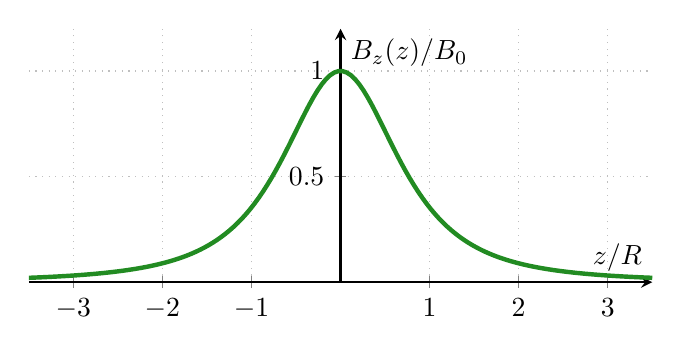
\begin{tikzpicture}
        \begin{axis}[
            width=9.5cm, height=4.8cm,
            axis lines=middle,
            xmin=-3.5, xmax=3.5,
            ymin=0, ymax=1.2,
            xlabel={$z / R$},
            ylabel={$B_z(z) / B_0$},
            xtick={-3, -2, -1, 0, 1, 2, 3},
            ytick={0, 0.5, 1.0},
            grid=both,
            grid style={dotted, gray!50},
            thick
        ]
            \addplot[domain=-3.5:3.5, samples=150, ultra thick, ForestGreen] {1 / (1 + x^2)^(1.5)};
        \end{axis}
    \end{tikzpicture}
    \caption{Normalized axial magnetic field profile $B_z(z)/B_0 = (1 + (z/R)^2)^{-3/2}$.}
    \label{fig:b_profile_plot}
\end{figure}

---

\subsection{Continuous Current Generalizations}
\label{sec:continuous_currents}

The Biot-Savart law generalizes to 2D surface current densities $\vb{K}$ and 3D volume current densities $\vb{J}$:

\begin{definition}{Generalized Biot-Savart Laws}{generalized_biot_savart}
\begin{align}
    \vb{B}(\vb{r}_P) &= \frac{\mu_0}{4\pi} \int_{\mathcal{S}} \frac{\vb{K}(\vb{r}') \times \vu{r}^*}{{r^*}^2}\,da' \quad &\text{(Surface Currents)} \\
    \vb{B}(\vb{r}_P) &= \frac{\mu_0}{4\pi} \int_{\mathcal{V}} \frac{\vb{J}(\vb{r}') \times \vu{r}^*}{{r^*}^2}\,d\tau' \quad &\text{(Volume Currents)}
\end{align}
\end{definition}

\begin{remark}[Single Moving Point Charge]
One often sees the expression $\vb{B} \approx \frac{\mu_0}{4\pi} \frac{q \vb{v} \times \vu{r}^*}{{r^*}^2}$. This is \textbf{not} strictly exact. An isolated moving charge does not constitute a steady current ($\div\vb{J} \neq 0$), generating an intrinsically time-dependent electric field ($\pdv{\vb{E}}{t} \neq \vb{0}$). This expression is valid only as a quasi-static, non-relativistic approximation ($v \ll c$) where retardation effects are negligible.
\end{remark}

---

\subsection{The Divergence and Curl of $\vb{B}$}
\label{sec:div_curl_b}

We now derive the field equations of magnetostatics directly from the Biot-Savart law:
\begin{equation}
    \vb{B}(\vb{r}) = \frac{\mu_0}{4\pi} \int_{\mathcal{V}} \vb{J}(\vb{r}') \times \frac{\vb{r} - \vb{r}'}{\abs{\vb{r} - \vb{r}'}^3}\,d\tau'
\end{equation}
where $\vb{r} = (x,y,z)$ denotes field coordinates and $\vb{r}' = (x',y',z')$ denotes source coordinates. Differential operators $\grad$ act strictly on unprimed coordinates $\vb{r}$.

\subsubsection{The Divergence of $\vb{B}$}

\begin{theorem}{Absence of Magnetic Monopoles (Gauss's Law for Magnetism)}{div_b_zero}
The divergence of any static magnetic field is identically zero:
\begin{equation}
    \div\vb{B} = 0
\end{equation}
\end{theorem}

\begin{proofbox}
Taking the divergence with respect to unprimed coordinates:
\begin{equation}
    \div\vb{B} = \frac{\mu_0}{4\pi} \int \div\qty(\vb{J}(\vb{r}') \times \frac{\vu{r}^*}{{r^*}^2})\,d\tau'
\end{equation}
Using the vector identity $\div(\vb{u} \times \vb{v}) = \vb{v} \cdot (\curl\vb{u}) - \vb{u} \cdot (\curl\vb{v})$:
\begin{equation}
    \div\qty(\vb{J}(\vb{r}') \times \frac{\vu{r}^*}{{r^*}^2}) = \frac{\vu{r}^*}{{r^*}^2} \cdot \qty(\grad \times \vb{J}(\vb{r}')) - \vb{J}(\vb{r}') \cdot \qty(\grad \times \frac{\vu{r}^*}{{r^*}^2})
\end{equation}
We examine both terms:
\begin{enumerate}
    \item $\grad \times \vb{J}(\vb{r}') = \vb{0}$, because $\vb{J}(\vb{r}')$ depends exclusively on primed coordinates.
    \item $\grad \times \qty(\frac{\vu{r}^*}{{r^*}^2}) = -\grad \times \grad\qty(\frac{1}{r^*}) = \vb{0}$, since the curl of any gradient field is identically zero.
\end{enumerate}
Both terms vanish identically, yielding:
\begin{equation}
    \div\vb{B} = 0
\end{equation}
\end{proofbox}

\subsubsection{The Curl of $\vb{B}$ and Ampère's Law}

\begin{theorem}{Ampère's Law in Differential Form}{amperes_law_diff}
For steady currents, the curl of the magnetic field satisfies:
\begin{equation}
    \curl\vb{B} = \mu_0 \vb{J}
\end{equation}
\end{theorem}

\begin{proofbox}
Applying the curl operator to the Biot-Savart law:
\begin{equation}
    \curl\vb{B} = \frac{\mu_0}{4\pi} \int \grad \times \qty(\vb{J}(\vb{r}') \times \frac{\vu{r}^*}{{r^*}^2})\,d\tau'
\end{equation}
Employing the vector product rule $\grad \times (\vb{u} \times \vb{v}) = \vb{u}(\div\vb{v}) - \vb{v}(\div\vb{u}) + (\vb{v}\cdot\grad)\vb{u} - (\vb{u}\cdot\grad)\vb{v}$:
\begin{equation}
    \grad \times \qty(\vb{J} \times \frac{\vu{r}^*}{{r^*}^2}) = \vb{J}\qty(\grad \cdot \frac{\vu{r}^*}{{r^*}^2}) - \qty(\vb{J} \cdot \grad)\frac{\vu{r}^*}{{r^*}^2}
\end{equation}
The remaining two gradient terms vanish because $\grad$ does not act on $\vb{J}(\vb{r}')$.

\textbf{Step 1: Evaluation of the second term.}
Using the identity $\grad f(r^*) = -\grad' f(r^*)$ from the chain rule:
\begin{equation}
    -(\vb{J} \cdot \grad)\frac{\vu{r}^*}{{r^*}^2} = (\vb{J} \cdot \grad')\frac{\vu{r}^*}{{r^*}^2}
\end{equation}
For each Cartesian component $i \in \{x,y,z\}$:
\begin{equation}
    \qty[(\vb{J} \cdot \grad')\frac{x_i - x_i'}{{r^*}^3}] = \div'\qty[\frac{x_i - x_i'}{{r^*}^3} \vb{J}] - \frac{x_i - x_i'}{{r^*}^3}\qty(\div'\vb{J})
\end{equation}
For steady currents, $\div'\vb{J} = 0$. Integrating the divergence term over all space and applying the divergence theorem:
\begin{equation}
    \int_{\mathcal{V}} \div'\qty[\frac{x_i - x_i'}{{r^*}^3} \vb{J}]\,d\tau' = \oint_{\partial \mathcal{V}} \frac{x_i - x_i'}{{r^*}^3} (\vb{J} \cdot d\vb{a}') = 0
\end{equation}
since the boundary $\partial\mathcal{V}$ can be taken outside the localized current distribution where $\vb{J} = \vb{0}$.

\textbf{Step 2: Evaluation of the first term.}
Using the fundamental distributional identity:
\begin{equation}
    \grad \cdot \qty(\frac{\vu{r}^*}{{r^*}^2}) = 4\pi \delta^3(\vb{r} - \vb{r}')
\end{equation}
Substituting this back into the volume integral:
\begin{equation}
    \curl\vb{B} = \frac{\mu_0}{4\pi} \int \vb{J}(\vb{r}') \qty(4\pi \delta^3(\vb{r} - \vb{r}'))\,d\tau' = \mu_0 \vb{J}(\vb{r})
\end{equation}
\end{proofbox}

\begin{proposition}{Ampère's Law in Integral Form}{ampere_integral}
Applying Stokes' theorem to an open surface $\mathcal{S}$ bounded by closed contour $\mathcal{C}$:
\begin{equation}
    \int_{\mathcal{S}} (\curl\vb{B}) \cdot d\vb{a} = \oint_{\mathcal{C}} \vb{B} \cdot d\vb{\ell} = \mu_0 \int_{\mathcal{S}} \vb{J} \cdot d\vb{a}
\end{equation}
which yields:
\begin{equation}
    \oint_{\mathcal{C}} \vb{B} \cdot d\vb{\ell} = \mu_0 I_{\mathrm{enc}}
\end{equation}
where $I_{\mathrm{enc}}$ is the total net current puncturing the surface bounded by the Amperian loop $\mathcal{C}$.
\end{proposition}

---

\subsection{Applications of Ampère's Law}
\label{sec:ampere_applications}

Ampère's law provides a highly efficient method for determining magnetic fields in systems exhibiting high degrees of symmetry (cylindrical, planar, or solenoidal).

\subsubsection{Infinite Straight Current-Carrying Wire}

Consider an infinitely long, thin wire lying along the $z$-axis carrying steady current $I$.

\begin{figure}[htbp]
    \centering
    \begin{tikzpicture}[scale=1.1, >=Stealth]
        % Wire
        \draw[very thick, ->, ForestGreen] (-3.0,0) -- (3.0,0) node[right] {$I$};
        
        % Amperian loop
        \draw[thick, Orange!90!black] (0,0) ellipse (0.7cm and 1.8cm);
        \draw[thick, ->, Orange!90!black] (0.7,0) -- (0.7,0.1);
        \draw[thick, ->, Orange!90!black] (-0.7,0) -- (-0.7,-0.1);
        
        % Radius s
        \draw[thick, ->] (0,0) -- (0,1.8) node[midway, right] {$s$};
        \node[Orange!90!black, above] at (0,1.8) {Amperian loop};
        
        % Field direction
        \node[Orange!90!black, below left] at (-0.7,-1.0) {$\vb{B}$};
    \end{tikzpicture}
    \caption{Circular Amperian loop of radius $s$ concentric with an infinite straight current $I$.}
    \label{fig:straight_wire_ampere}
\end{figure}

By cylindrical symmetry:
\begin{equation}
    \vb{B} = B_\phi(s)\,\vu*{\phi}
\end{equation}
Integrating around a circular Amperian loop of radius $s$:
\begin{equation}
    \oint_{\mathcal{C}} \vb{B} \cdot d\vb{\ell} = B_\phi(s) \oint d\ell = B_\phi(s) (2\pi s) = \mu_0 I_{\mathrm{enc}} = \mu_0 I
\end{equation}
Solving directly for the magnetic field:
\begin{equation}
    \vb{B}(s) = \frac{\mu_0 I}{2\pi s}\,\vu*{\phi}
\end{equation}

\subsubsection{Infinite Uniform Surface Current Sheet}

Consider an infinite conductive sheet lying in the $xy$-plane carrying uniform surface current density $\vb{K} = K\,\vu{x}$.

\begin{figure}[htbp]
    \centering
    \begin{tikzpicture}[scale=1.1, >=Stealth]
        % Current sheet in xy plane
        \fill[ForestGreen!15] (-2.2,-1.0) -- (1.5,-1.0) -- (3.2,1.2) -- (-0.5,1.2) -- cycle;
        \draw[thin, ForestGreen!60!black] (-2.2,-1.0) -- (1.5,-1.0) -- (3.2,1.2) -- (-0.5,1.2) -- cycle;
        
        % Surface current vector
        \draw[ultra thick, ->, ForestGreen] (-0.2,0.6) -- (-1.4,-0.4) node[midway, above left] {$\vb{K} = K\,\vu{x}$};
        
        % Axes
        \draw[thin, ->] (0,0) -- (0,2.4) node[above] {$z$};
        \draw[thin, ->] (0,0) -- (2.8,0) node[right] {$y$};
        \draw[thin, ->] (0,0) -- (-1.2,-1.0) node[below left] {$x$};
        
        % Rectangular Amperian loop in yz plane
        \coordinate (L1) at (0.8,-0.9);
        \coordinate (L2) at (1.8,-0.9);
        \coordinate (L3) at (1.8,0.9);
        \coordinate (L4) at (0.8,0.9);
        
        \draw[thick, Orange!90!black] (L1) -- (L2) -- (L3) -- (L4) -- cycle;
        \draw[thick, ->, Orange!90!black] (L1) -- ($(L1)!0.5!(L2)$);
        \draw[thick, ->, Orange!90!black] (L3) -- ($(L3)!0.5!(L4)$);
        \draw[<->] (0.8,-1.1) -- (1.8,-1.1) node[midway, below] {$\ell$};
        \node[Orange!90!black, right] at (1.8,0.5) {Amperian loop};
    \end{tikzpicture}
    \caption{Rectangular Amperian loop perpendicular to an infinite current sheet carrying $\vb{K} = K\,\vu{x}$.}
    \label{fig:current_sheet_ampere}
\end{figure}

\begin{enumerate}
    \item \textbf{Symmetry analysis:}
    \begin{itemize}
        \item Field components along $x$ vanish identically: $\vb{K} \parallel \vu{x} \implies (\vb{K} \times \vu{r}^*)_x = 0 \implies B_x = 0$.
        \item Any vertical component $B_z$ from a current filament at $+y$ is exactly cancelled by the filament at $-y \implies B_z = 0$.
        \item By the right-hand rule, $\vb{B}$ points in the $-\vu{y}$ direction above the sheet ($z > 0$) and in the $+\vu{y}$ direction below the sheet ($z < 0$).
    \end{itemize}
    \item \textbf{Amperian circulation:} Choose a rectangular loop of width $\ell$ spanning from $-z$ to $+z$ parallel to the $yz$-plane. The vertical segments contribute nothing because $\vb{B} \perp d\vb{\ell}$. The two horizontal segments give:
    \begin{equation}
        \oint \vb{B} \cdot d\vb{\ell} = B \ell + B \ell = 2 B \ell
    \end{equation}
    \item \textbf{Enclosed current:} $I_{\mathrm{enc}} = K \ell$.
\end{enumerate}
Equating both sides via Ampère's law:
\begin{equation}
    2 B \ell = \mu_0 K \ell \implies B = \frac{\mu_0 K}{2}
\end{equation}
Accounting for vector orientation:
\begin{equation}
    \vb{B}(z) = \begin{cases}
        -\dfrac{\mu_0 K}{2}\,\vu{y}, & z > 0 \\[8pt]
        +\dfrac{\mu_0 K}{2}\,\vu{y}, & z < 0
    \end{cases}
    \label{eq:sheet_b_field}
\end{equation}

\begin{remark}[Discontinuity Across a Surface Current]
Notice that the magnetic field experiences a finite jump discontinuity across the sheet:
\begin{equation}
    \Delta\vb{B} = \vb{B}_{\mathrm{above}} - \vb{B}_{\mathrm{below}} = -\mu_0 K\,\vu{y} = \mu_0 (\vb{K} \times \vu{n})
\end{equation}
where $\vu{n} = \vu{z}$ is the unit normal to the surface. This is the magnetic analog to the electrostatic discontinuity $\Delta\vb{E} = \frac{\sigma}{\epsilon_0}\vu{n}$.
\end{remark}

---

\subsection{Summary of Week 8 Core Results}

\begin{table}[htbp]
    \centering
    \renewcommand{\arraystretch}{1.5}
    \small
    \begin{tabular}{lll}
        \hline
        \textbf{Physical Concept} & \textbf{Mathematical Formulation} & \textbf{Physical Meaning / Scope} \\
        \hline
        Lorentz Force & $\vb{F} = Q(\vb{E} + \vb{v}\times\vb{B})$ & Fundamental force on point charge $Q$ \\
        Magnetic Work & $dW_{\mathrm{mag}} = \vb{F}_{\mathrm{mag}} \cdot \vb{v}\,dt = 0$ & Magnetic fields do zero mechanical work \\
        Cyclotron Frequency & $\omega_c = \frac{\abs{q}B}{m}$ & Independent of particle speed and radius \\
        Wire Force & $d\vb{F} = I\,d\vb{s} \times \vb{B}$ & Force on macroscopic steady current line \\
        Closed Loop Force & $\oint_{\mathcal{C}} d\vb{s} \times \vb{B} = \vb{0}$ & Net translational force vanishes in uniform $\vb{B}$ \\
        Magnetic Dipole Moment & $\bm{\mu} = N I \vb{A}$ & Direct analog to electric dipole moment \\
        Magnetic Torque & $\bm{\tau} = \bm{\mu} \times \vb{B}$ & Tends to align dipole moment with ambient field \\
        Biot-Savart Law & $d\vb{B} = \frac{\mu_0}{4\pi}\frac{I\,d\vb{s}\times\vu{r}^*}{{r^*}^2}$ & Primary fundamental field source integral \\
        Absence of Monopoles & $\div\vb{B} = 0$ & Magnetic field lines form continuous closed loops \\
        Ampère's Law (Diff.) & $\curl\vb{B} = \mu_0 \vb{J}$ & Fundamental field equation for steady currents \\
        Ampère's Law (Int.) & $\oint_{\mathcal{C}} \vb{B}\cdot d\vb{\ell} = \mu_0 I_{\mathrm{enc}}$ & Efficient calculation for symmetric distributions \\
        \hline
    \end{tabular}
    \caption{Synoptic summary of foundational formulas and theorems established in Week 8.}
    \label{tab:week8_summary}
\end{table}

% =========================================================================
% END OF WEEK 8 TRANSCRIPT
% =========================================================================